\documentclass{beamer}

\mode<presentation> {
\usetheme{CambridgeUS}
}

\usepackage{algorithmicx}
\usepackage{algorithm}
\usepackage{algpseudocode}
\usepackage{amsmath}
\usepackage{amssymb}
\usepackage{hyperref}

\graphicspath{{images/}}

%-------------------------------------------------------------------------------
% Presentation meta
%-------------------------------------------------------------------------------

\title{Multi-step RL: Unifying Algorithm}

\author{Kirill Bobyrev}

\date{\today}

\begin{document}

\begin{frame}
  \titlepage
\end{frame}

\begin{frame}
  \frametitle{Plan}
  \tableofcontents
\end{frame}

%-------------------------------------------------------------------------------
% Slides
%-------------------------------------------------------------------------------

%-------------------------------------------------------------------------------
\section{Introduction}
%-------------------------------------------------------------------------------

\begin{frame}
  \frametitle{Results}
  Introducing algorithm $Q(\sigma)$ with following properties
  \begin{itemize}
    \item Model-free
    \item Can be trained both off- and on-policy
    \item Uses $n$-step backup rule
    \item Generalizes a huge number of existing algorithms while subsuming them
      as special cases
    \item Performs better given a reasonable choice of hyperparameter $\sigma$
  \end{itemize}
\end{frame}

%-------------------------------------------------------------------------------
\section{From MC and one-step TD to multi-step Bootstrapping}
%-------------------------------------------------------------------------------

\begin{frame}
  \frametitle{Monte Carlo methods}
  \begin{itemize}
    \item Sample many episodes
    \item MC every-visit backup: $V(S_t) \leftarrow V(S_t) +
      \alpha[G_t - V(S_t)]$
    \item Does not need environment model
  \end{itemize}
\end{frame}

\begin{frame}
  \frametitle{TD methods}
  \begin{itemize}
    \item Combines Monte Carlo and Dynamic Programming
    \item Does not need environment model
    \item Uses bootstrapping for updates
    \item Sample many steps instead of methods
    \item One-step TD backup: $V(S_t) \leftarrow V(S_t) +
      \alpha[R_t - \gamma V(S_t)]$
  \end{itemize}
\end{frame}

%-------------------------------------------------------------------------------
\section{$n$-step methods}
%-------------------------------------------------------------------------------

%-------------------------------------------------------------------------------
\subsection{1-step into $n$-steps transition}
%-------------------------------------------------------------------------------

\begin{frame}
  \frametitle{From 1-step to $n$-step}
  Define multi-step return for TD: $G_{t : t + n} \overset{\cdot}{=} R_{t + 1} +
    \gamma R_{t + 2} + \ldots + \gamma^{n - 1} R_{t + n} +
    \gamma^n V_{t + n - 1}(S_{t + n})$

  Using this multi-step return:
  \begin{itemize}
    \item Monte Carlo backup uses $G_{t : T}$
    \item One-step TD backup uses $G_{t : t + 1}$
  \end{itemize}

  $n$-step TD: $V_{t + n}(S_t) \overset{\cdot}{=} V_{t + n - 1}(S_t) +
    \alpha [G_{t : t + n} - V_{t + n - 1}(S_t)]$

  $Q(\sigma)$ is based on $n$-step Sarsa and $n$-step Tree Backup
\end{frame}

%-------------------------------------------------------------------------------
\subsection{Backups overview}
%-------------------------------------------------------------------------------

\begin{frame}
  \frametitle{Backups: From one-step TD to MC}
  \begin{figure}
    \centering
    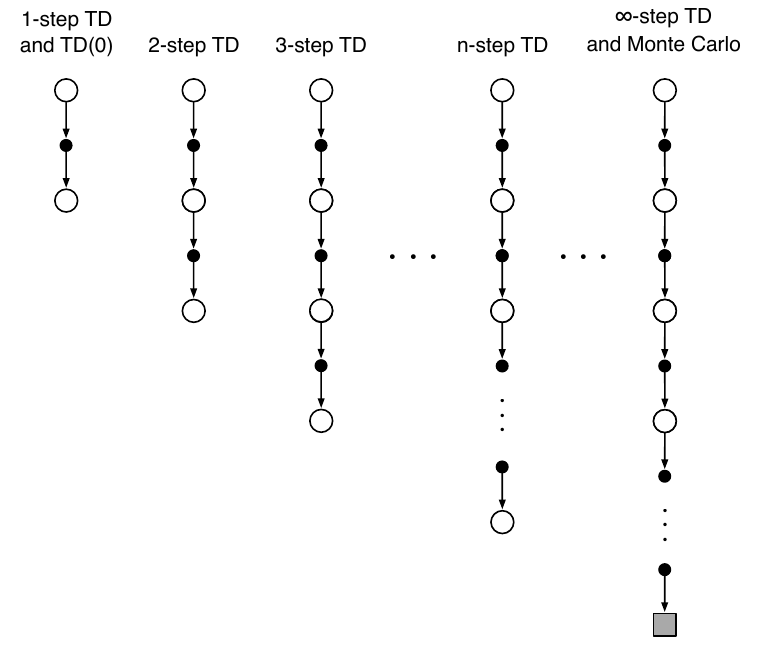
\includegraphics[height=0.7 \textheight]{one_step_to_multi_step}
    \caption{Backup schemes comparison: from $1$ step in TD(0) to $\infty$
      steps in Monte Carlo methods}
  \end{figure}
\end{frame}

\begin{frame}
  \frametitle{$n$-step Sarsa}
  Transition from one-step Sarsa to $n$-step version is straightforward:
  $$G_{t : t + n} \overset{\cdot}{=} R_{t + 1} + \gamma R_{t + 2} + \ldots +
    \gamma^{n -1} R_{t + n} + \gamma^n Q_{t + n - 1}(S_{t + n}, A_{t + n})$$
  The update rule is transformed as follows:
  $$Q_{t + n}(S_t, A_t) \overset{\cdot}{=} Q_{t + n - 1}(S_t, A_t) +
    \alpha [G_{t : t + n} - Q_{t + n - 1}(S_t, A_t)$$
  Generalizing Expected Sarsa would modify the error definition by a small
  margin:
  $$\delta^{S}_t = R_{t + 1} + \gamma Q(S_{t + 1}, A_{t + 1}) - Q(S_t, A_t)$$
  $$\delta^{ES}_t \overset{\cdot}{=} R_{t + 1} +
    \gamma \sum_{a} \pi(a | S_{t + 1}) Q_t(S_{t + 1}, a) - Q_{t - 1}(S_t, A_t)$$
  Therefore we obtain Expected Sarsa return:
  $$G_{t : t + n} \overset{\cdot}{=} R_{t + 1} + \ldots +
    \gamma^{n -1} R_{t + n} + \gamma^n \sum_{a} \pi(a | S_{t + n})
      Q_{t + n - 1}(S_{t + n}, A_{t + n})$$
\end{frame}

\begin{frame}
  \frametitle{Sarsa off-policy learning}
  \begin{itemize}
    \item $\pi$ is greedy policy for the current action-value-function estimate
    \item $\mu$ is exploratory policy, perhaps $\varepsilon$-greedy
  \end{itemize}
  Goal: learn value function for $\pi$ while following $\mu$
  Solution: use importance sampling ratio and modify update rule
  $$\rho_{t : t + n} = \prod_{k = t}^{\min{t + n, T - 1}}
    \frac{\pi(A_k | S_k)}{\mu(A_k | S_k)}$$
  $$Q_{t + n}(S_t, A_t) \overset{\cdot}{=} Q_{t + n - 1}(S_t, A_t) +
    \alpha \rho_{t + 1 : t + n - 1} [G_{t : t + n} - Q_{t + n - 1}(S_t, A_t)]$$
\end{frame}

\begin{frame}
  \frametitle{$n$-step Sarsa and Expected Sarsa backup mechanisms}
  \begin{figure}
    \centering
    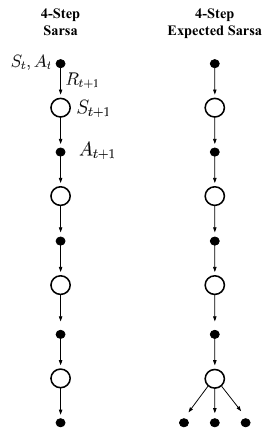
\includegraphics[height=0.6 \textheight]{sarsa_backup}
    \caption{Backup schemes for Sarsa and Expected Sarsa with $n = 4$. Expected
      Sarsa computes return expectation using all values of the valid outgoing
      states on the last step.}
  \end{figure}
\end{frame}

\begin{frame}
  \frametitle{Tree Backup: off-policy without Importance Sampling}
  Tree Backup is the multi-step generalization of Expected Sarsa:
  $$G_{t : t + 1} \overset{\cdot}{=} R_{t + 1} +
    \gamma \sum_{a} \pi(a | S_{t + 1}) Q_t(S_{t + 1}, a) = \delta^{ES}_t
    + Q_{t - 1}(S_{t + 1}, a)$$
  Hence $n$-step return of Tree Backup is a sum of TD errors:
  % TODO: Check that the following error is indeed \delta^ES.
  $$G_{t : t + n} \overset{\cdot}{=} Q_{t -1}(S_t, A_t) +
    \sum_{k = t}^{\min{t + n - 1, T - 1}} \delta_k^{ES} \prod_{i = t + 1}^k
    \gamma \pi(A_i | S_i)$$
  Taking update rule from $n$-step Sarsa:
  $$Q_{t + n}(S_t, A_t) \overset{\cdot}{=} Q_{t + n - 1}(S_t, A_t) +
    \alpha[G_{t : t + n} - Q_{t + n -1}(S_t, A_t)]$$
\end{frame}

\begin{frame}
  \frametitle{Tree Backup mechanism}
  \begin{figure}
    \centering
    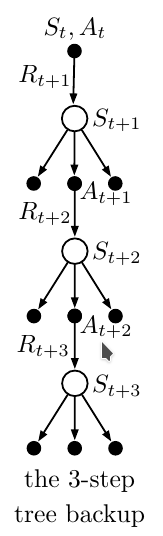
\includegraphics[height=0.7 \textheight]{tree_backup}
    \caption{Tree Backup calculates the expected return of each step using
      $\delta_t^{ES}$ at each timestep $t$}
  \end{figure}
\end{frame}

%-------------------------------------------------------------------------------
\section{$Q(\sigma)$ algorithm}
%-------------------------------------------------------------------------------

%-------------------------------------------------------------------------------
\subsection{Relation to other algorithms}
%-------------------------------------------------------------------------------

\begin{frame}
  \frametitle{Relation to other algorithms}
  Two families of multi-step algorithms:
  \begin{itemize}
    \item Algorithms that backup their actions and samples (Sarsa and
      Expected Sarsa)
    \item Algorithms that consider an expectation over all actions in their
      backup (Expected Sarsa and Tree Backup)
  \end{itemize}
  New parameter $\sigma \in [0, 1]$, which controls the degree of sampling at
  each step of the backup, unifies both families
\end{frame}

%-------------------------------------------------------------------------------
\subsection{Backups}
%-------------------------------------------------------------------------------

\begin{frame}
  \frametitle{Details}
  Error modification:
  \begin{align*}
    \delta_t^{\sigma}
      &= \sigma_{t+1} \delta_{t}^S + (1 - \sigma_{t + 1}) \delta_t^{ES} \\
      &= R_{t + 1} + \gamma [\sigma_{t + 1} Q_t(S_{t + 1}, A_{t + 1}) +
                          (1 - \sigma_{t+ 1}) V_{t + 1}] - Q_{t - 1}(S_t, A_t)
  \end{align*}
  Resulting return:
  $$G_{t}^{(n)} = Q_{t - 1}(S_t, A_t) + \sum_{k = t}^{\min{t + n - 1, T- 1}}
    \delta_k^{\sigma} \prod_{i = t + 1}^{k} \gamma
    [(1 - \sigma_i) \pi (A_i | S) + \sigma_i]$$
\end{frame}

\begin{frame}
  \frametitle{Backup comparisons}
  \begin{figure}
    \centering
    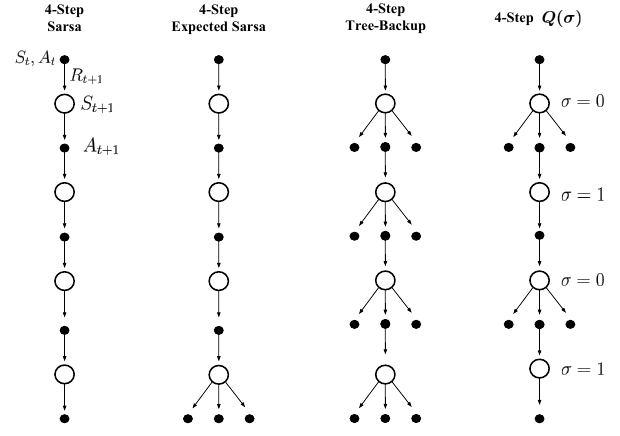
\includegraphics[width=0.6 \textwidth]{all_multi_step_backups}
    \caption{Backup mechanisms for the presented atomic multi-step algorithms
      with $n = 4$. $Q(\sigma)$ combines backup techniques of the previous
      algorithms}
  \end{figure}
\end{frame}

%-------------------------------------------------------------------------------
\subsection{Off-policy learning}
%-------------------------------------------------------------------------------

\begin{frame}
  \frametitle{$Q(\sigma)$ off-policy learning}
  \begin{itemize}
    \item Both base algorithms can be trained off-policy
    \item $Q(\sigma)$ importance sampling for off-policy learning combines the
    off-policy learning ideas for base algorithms
  \end{itemize}
  Learning policy $\pi$ while following $\mu$ can be achieved via introducing
  appropriate importance ratio:
  $$\rho_{t + 1}^{t + n} = \prod_{k = t + 1}^{\min{t + n - 1, T - 1}}
    (\sigma_k \frac{\pi(A_k | S_k)}{\mu(A_k | S_k)} + 1 - \sigma_k)$$
\end{frame}

%-------------------------------------------------------------------------------
\subsection{Algorithm details}
%-------------------------------------------------------------------------------

\begin{frame}
  \frametitle{Algorithm description}
  \scalebox{0.8}{
  \begin{minipage}{\linewidth}
  \begin{algorithmic}[1]
    \State Initialize $S_0 \neq S_T$; select $A_0$ according to
      $\pi(. | S_0)$
    \State Store $S_0$, $A_0$ and $Q(S_0, A_0)$
    \For{$t\gets 0, T + n - 1$}
      \If{$t < T$}
        \State Take action $A_t$, get R, observe and store $S_{t + 1}$
        \If{$S_{t  +1}$ is $S_T$}
          \State Store $\delta_t^{\sigma} = R - Q(S_t, A_t)$
        \Else
          \State Select and store $A_{t + 1}$ according to $\pi(. | S_{t + 1}$
          \State Store $Q(S_{t + 1}, A_{t + 1})$, $\sigma_{t + 1}$,
            $\pi(A_{t + 1} | S_{t + 1})$
          \State Calculate and store $\delta_t^{\sigma}$
        \EndIf
      \EndIf
      \If{$t \geq n$}
        \State Calculate and store $G_t^{(n)}$
        \State Perform backup: $Q(S_t, A_t) \leftarrow S(_t, A_t) +
          \alpha [G_t^{(n)} - Q(S_t, A_t)]$
      \EndIf
  \EndFor
  \end{algorithmic}
  \end{minipage}
  }
\end{frame}

%-------------------------------------------------------------------------------
\section{Comparison}
%-------------------------------------------------------------------------------

\begin{frame}
  \frametitle{Comparing Sarsa, Tree Backup, $Q(0.5)$ and dynamic $\sigma$
    performance}
  \begin{figure}
  \centering
  \begin{minipage}{.48\textwidth}
    \centering
    \begin{figure}
      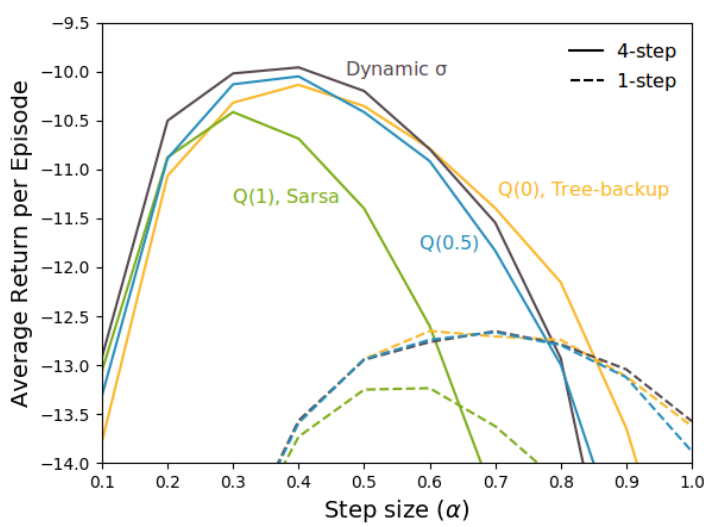
\includegraphics[width=\linewidth]{windy_gridworld_plot.png}
      \caption{Stochastic Windy Gridworld environment experiments. Results of
        the algorithms are averaged after 100 returns. $Q(\sigma)$ performed the
        best overall.}
    \end{figure}
  \end{minipage}
  \begin{minipage}{.48\textwidth}
    \centering
    \begin{figure}
      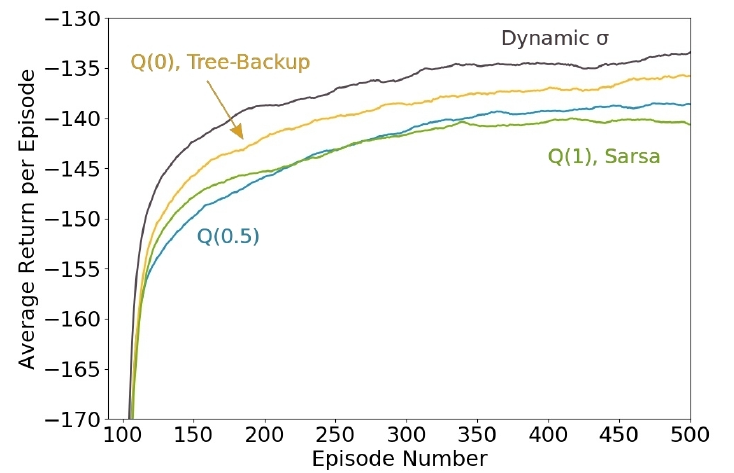
\includegraphics[width=\linewidth]{mountain_cliff_plot.png}
      \caption{Mountain cliff results. The plot shows that dynamic $\sigma$
        choosing strategy showed the best overall performance.}
    \end{figure}
  \end{minipage}
  \end{figure}
\end{frame}

%-------------------------------------------------------------------------------
\section{Future work}
%-------------------------------------------------------------------------------

\begin{frame}
  \frametitle{Room for improvements}
  \begin{itemize}
    \item Current definition of $Q(\sigma)$ is limited to the atomic multi-step
      case without eligibility traces, but it can be extended to use
      eligibility traces and compound backups
    \item Performance of $Q(\sigma)$ was only evaluated on on-policy problems,
      doing experiments with off-policy problems might be interesting
  \end{itemize}
\end{frame}

\begin{frame}
  \frametitle{Better $\sigma$ choosing}
  A trivial example of such strategies:
  \begin{itemize}
    \item Constant $\sigma = C$
    \item Altering $\sigma(t) = 1, 0, 1, 0, \ldots = [t \mod 2 = 0]$
    \item Random $\sigma(t) \sim \mathcal{U}[0, 1]$
    \item Decreasing or increasing over $t$ (between $0$ and $1$)
  \end{itemize}
  Other schemes for dynamically varying $\sigma$ could be investigated, for
  example a function of state, recently observed rewards or some measure of the
  learning progress.
\end{frame}

%-------------------------------------------------------------------------------
\section{Conclusion}
%-------------------------------------------------------------------------------

\begin{frame}
  \frametitle{Synopsis}
  Today we
  \begin{itemize}
    \item saw how $n$-step algorithms are derived from MC and one-step TD
      methods
    \item revised through Sarsa and Tree Backup
    \item were introduced to the $Q(\sigma)$ algorithm in MDP setting
    \item outlined the relation of presented algorithm to other $n$-step methods
    \item gained some intuition about algorithm structure
    \item compared $Q(\sigma)$ performance to its base algorithms
  \end{itemize}
\end{frame}

\begin{frame}
  \frametitle<presentation>{References}

  \begin{thebibliography}{10}

  \beamertemplatebookbibitems

  \beamertemplatearticlebibitems

  \bibitem{QSigma}
    Kristopher De Asis, J. Fernando Hernandez-Garcia, G. Zacharias Holland,
    Richard S. Sutton.
    \newblock {\href{https://arxiv.org/abs/1703.01327}{\em Multi-step
      Reinforcement Learning: A Unifying Algorithm}}.
    \newblock arXiv, 3 Mar 2017.

  \bibitem{RLBook} Richard S. Sutton, Andrew G. Barto.
    \newblock
    {\href{http://incompleteideas.net/sutton/book/the-book-2nd.html}{\em
      Reinforcement Learning: An Introduction}}.
    \newblock MIT Press, Cambridge, MA, 19 Jun 2017 Draft.

  \end{thebibliography}
\end{frame}

%-------------------------------------------------------------------------------

\begin{frame}
  \frametitle{Materials}
  \begin{center}
  Presentation, code and other materials are available in the GitHub
  \href{https://github.com/omtcyfz/talks/tree/master/n-step-q-sigma}{
    \textcolor{blue}{repository}}
  \end{center}
\end{frame}

%-------------------------------------------------------------------------------

\end{document}
